\chapter{System evaluation}
\label{System_evaluation}
In the previous chapter an algorithm was presented, which could be capable of classifying a set of consecutive samples into two groups: Activity detected or no activity detected. The algorithm is however dependent on several values which have not been determined yet as they might, or might not be dependent on the operating environment. This chapter will therefore focus on finding the ideal values for several test environments and compare them with each other.

This chapter will first present the measures used for evaluating the system. It will follow up with describing and evaluating several pedestrian test environments. It will then do the same for a scale model simulating a street and finalizes with summarising the results.

\section{Measures of evaluation}
The system will be evaluated on three different criteria: Precision, recall and and response time. Precision is defined in equation \ref{eq:precsion/recall} and gives us insight in how many situations the light would turn on unnecessarily. Recall is defined in equation \ref{eq:precsion/recall} and gives us insight in how often the light fails to turns on when an object passes by. 

\begin{equation}
\label{eq:precsion/recall}
Precision = \frac{TP}{TP + FP}
\quad
Recall = \frac{TP}{TP + FN}
\end{equation}
The precise repose time is impossible to determine with the used dataset, as the starting time of the event is not defined. It is however possible that if two different settings of algorithms trigger a detection, we compare the detection times with each other.

\section{Hallway Evaluation}
This section evaluates the system on detecting pedestrians walking by through a hallway. It will first explain the test set-up and procedure, followed by a section showing the ideally found algorithm settings and their detection results.

\subsection{Test set-up}

\begin{figure}
	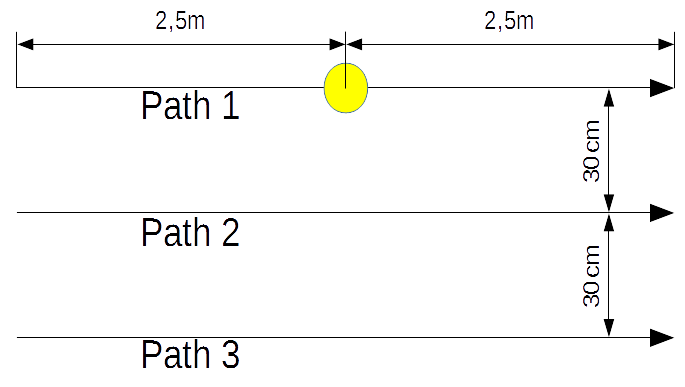
\includegraphics[width=\textwidth]{pics/Evaluation_paths.png}
	\caption{The three paths the test subjects had to walk underneath the light.}
	\label{fig:Evaluation_paths}
\end{figure}

\begin{figure}
	\centering     %%% not \center
	\label{fig:TestPicture}
	\subfigure[Indoor]{\label{fig:setup_a}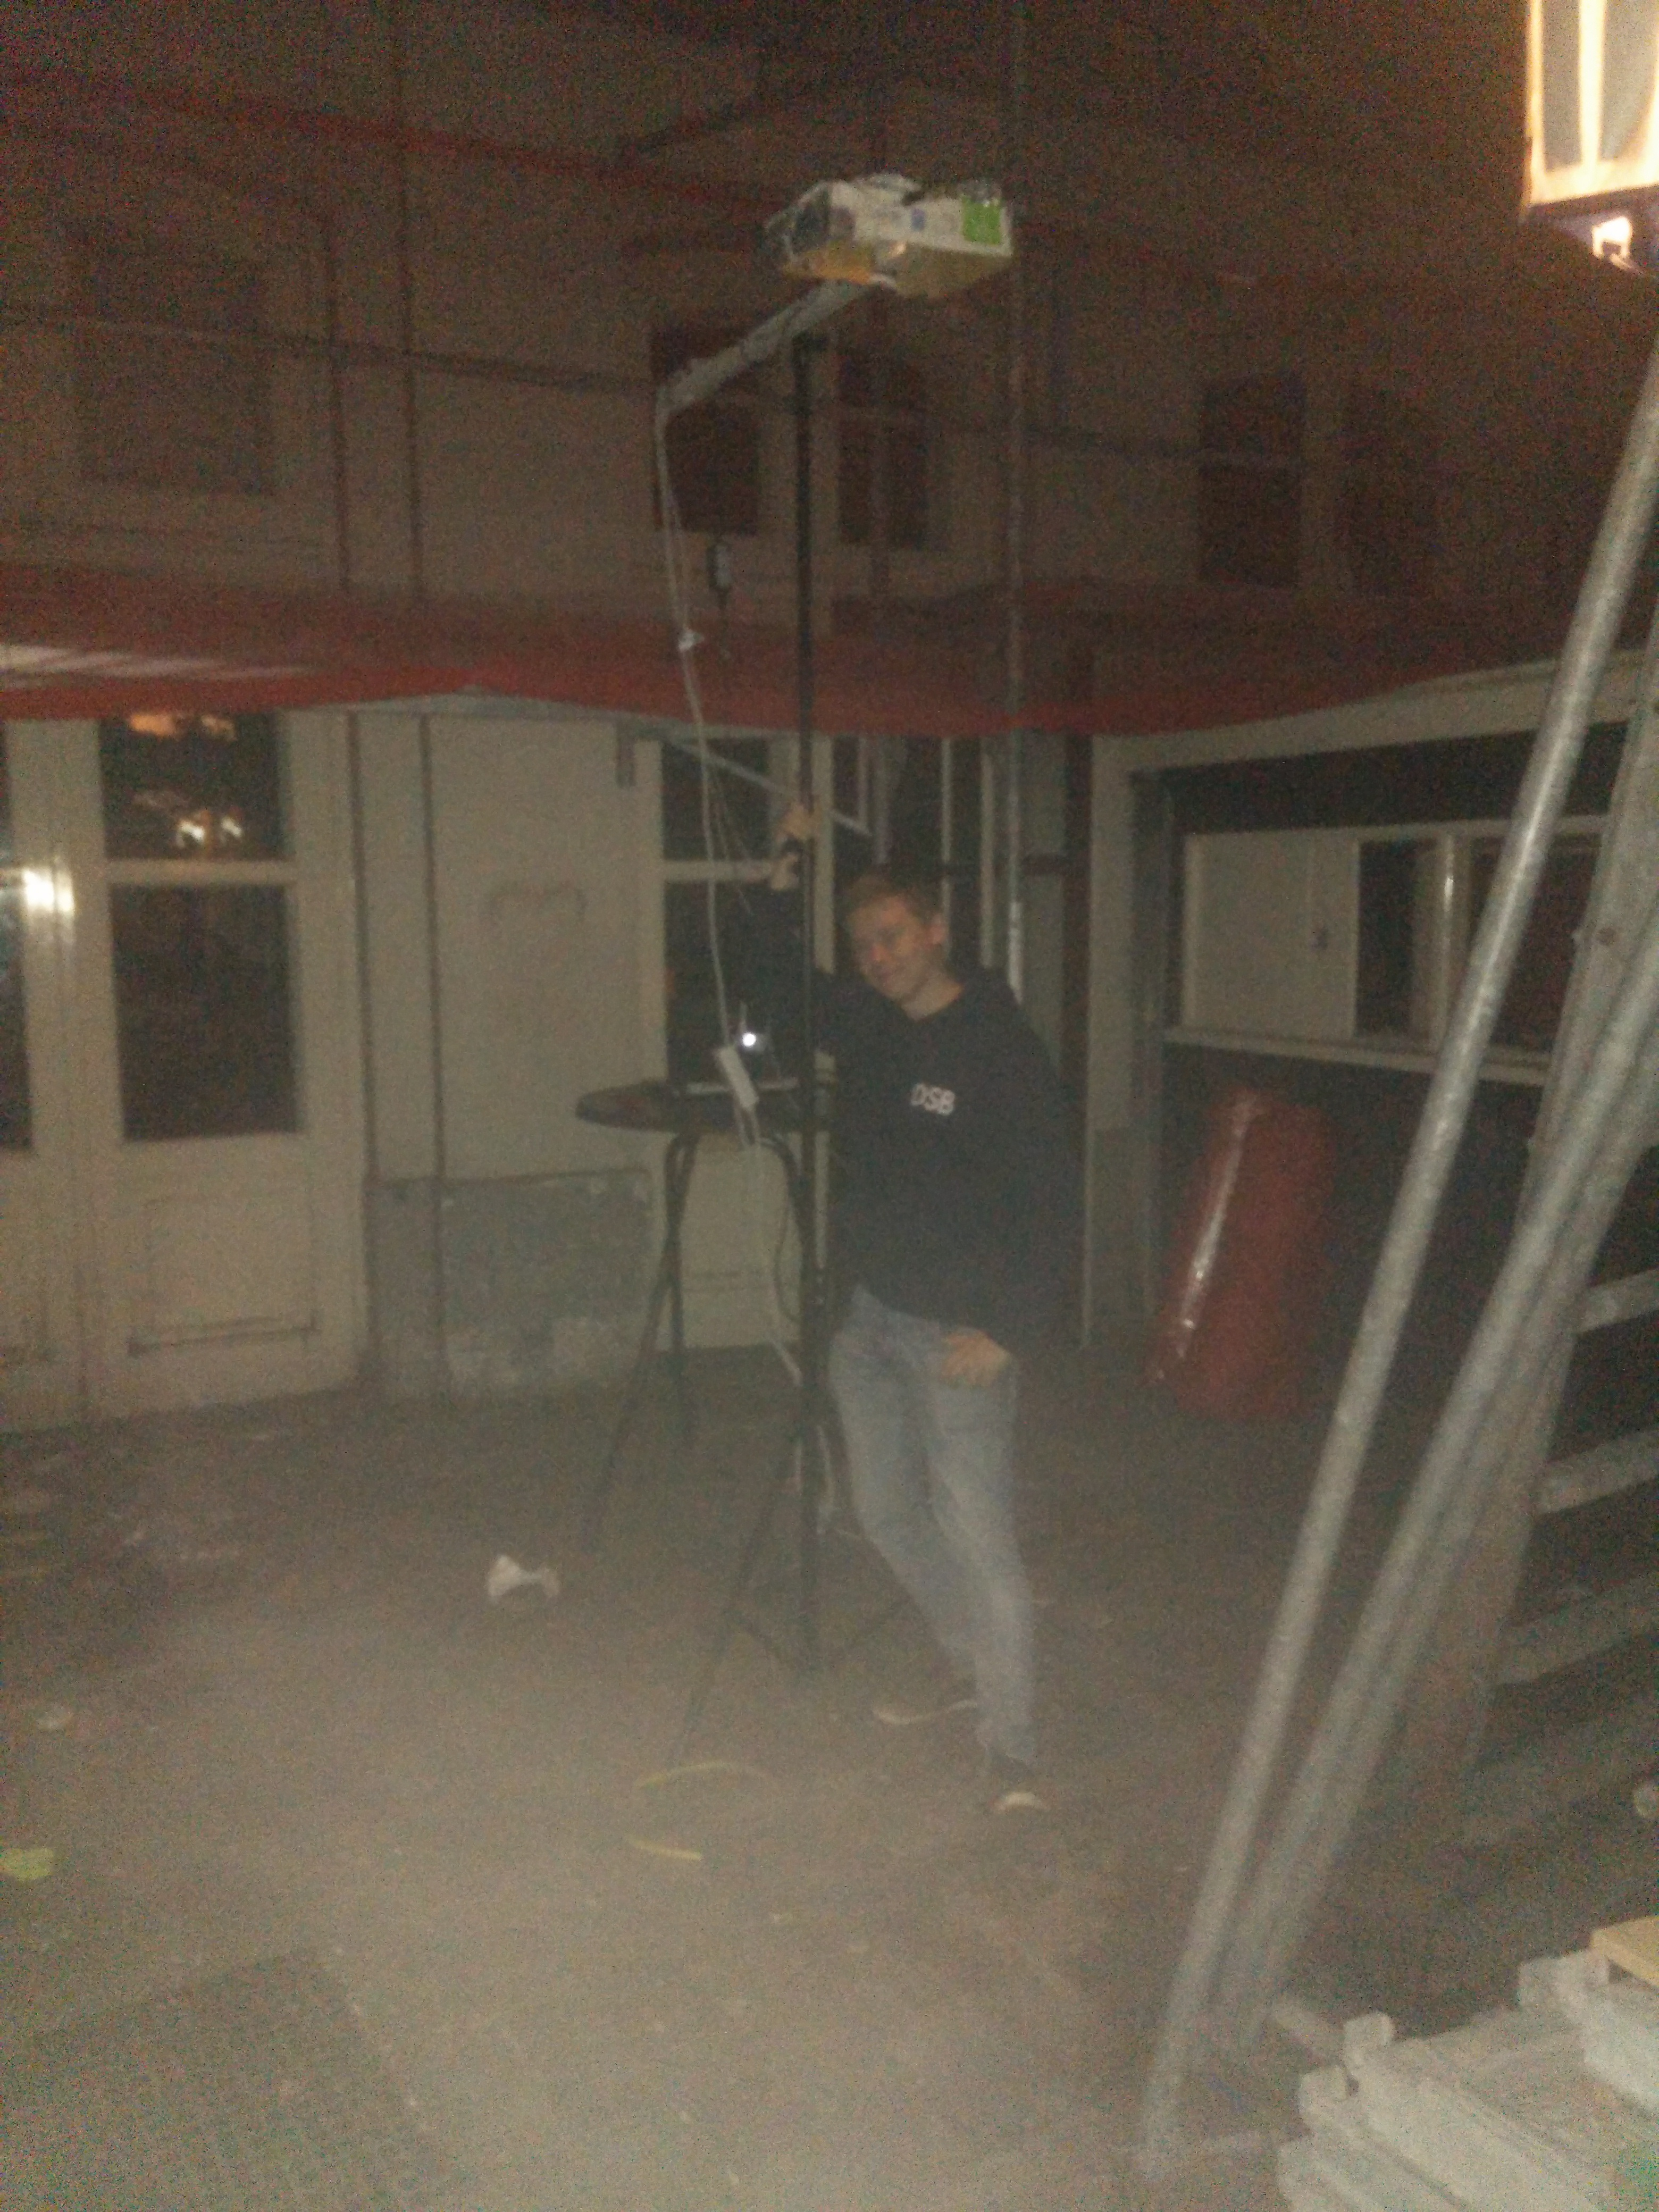
\includegraphics[width=60mm]{pics/Setup_outdoor.jpg}}
	\subfigure[Outdoor]{\label{fig:setup_b}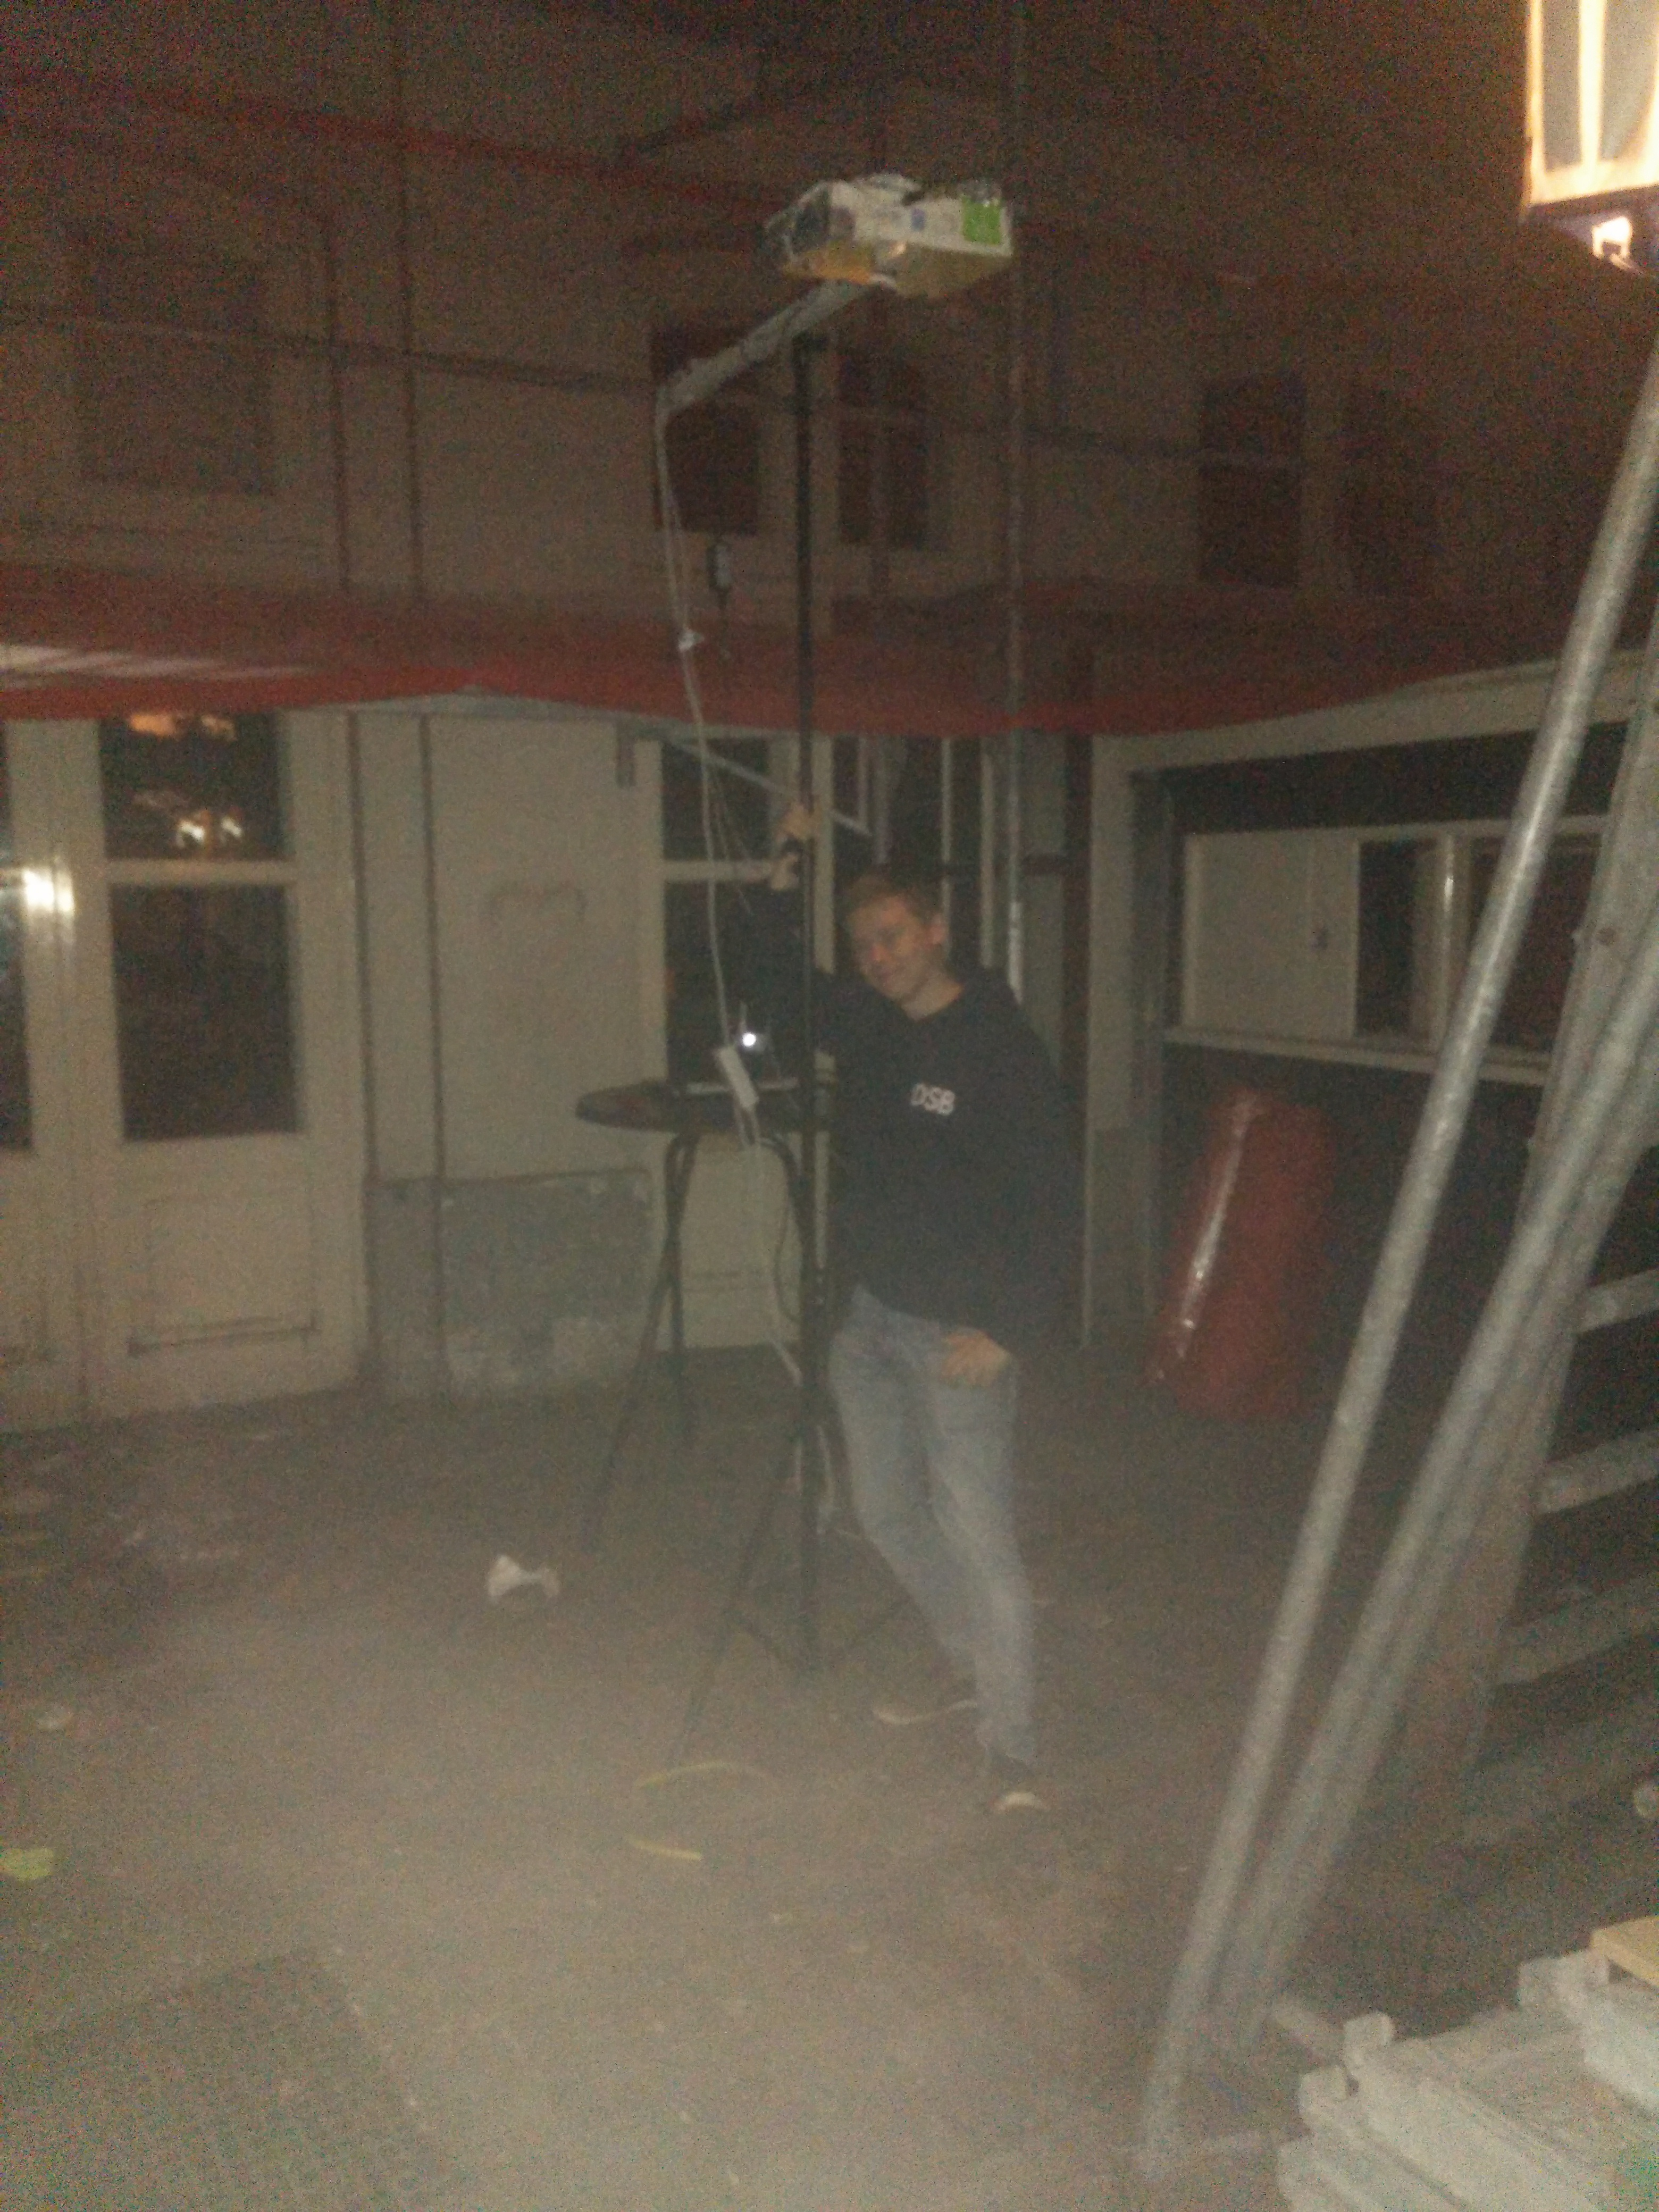
\includegraphics[width=60mm]{pics/Setup_outdoor.jpg}}
	\caption{Pictures of the test set-up indoor (a) and outdoor (b). The light was suspended at 2.6m high.}
\end{figure}

\subsection{Results}

\section{Street}
This section evaluates the system on detecting cars driving by on a road. It will first explain the test set-up and procedure, followed by a section showing the ideally found algorithm settings and their detection results.
\subsection{Test set-up}
\subsection{Results}

\section{Conclusion}